\hypertarget{histogram__data_8c}{
\section{bin/histogram\_\-data.c File Reference}
\label{histogram__data_8c}\index{bin/histogram\_\-data.c@{bin/histogram\_\-data.c}}
}
Edge length histogram data collector. 

{\tt \#include \char`\"{}arrow.h\char`\"{}}\par
{\tt \#include $<$getopt.h$>$}\par


Include dependency graph for histogram\_\-data.c:\nopagebreak
\begin{figure}[H]
\begin{center}
\leavevmode
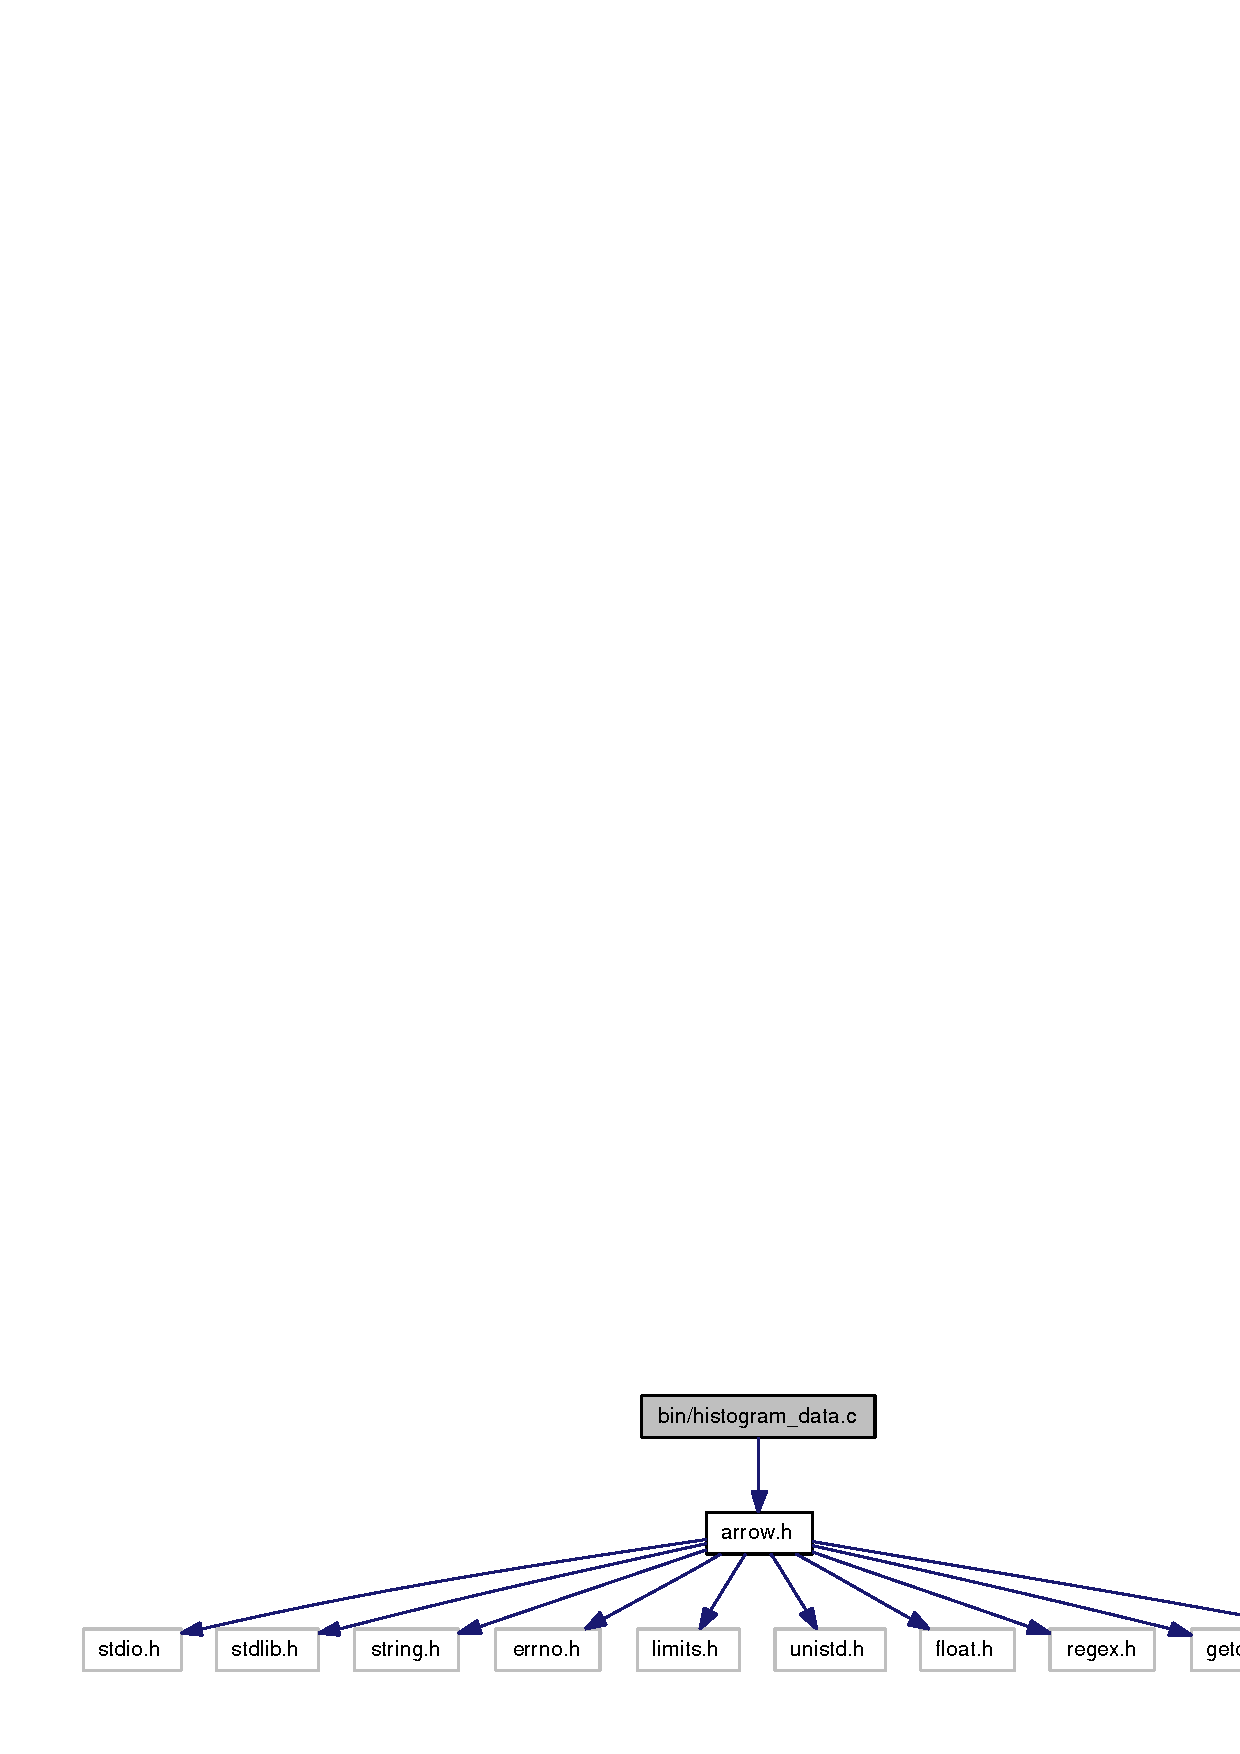
\includegraphics[width=257pt]{histogram__data_8c__incl}
\end{center}
\end{figure}
\subsection*{Functions}
\begin{CompactItemize}
\item 
void \hyperlink{histogram__data_8c_853216ac51aa181669ff4d3de74058a7}{print\_\-help} ()
\begin{CompactList}\small\item\em Prints help/usage message. \item\end{CompactList}\item 
void \hyperlink{histogram__data_8c_6302aaae12249e8ea16bfdc7de892f21}{print\_\-version} ()
\begin{CompactList}\small\item\em Prints version message. \item\end{CompactList}\item 
void \hyperlink{histogram__data_8c_e5ad5cbeccaedc03a48d3c7eaa803e79}{print\_\-usage} ()
\begin{CompactList}\small\item\em Prints usage message. \item\end{CompactList}\item 
void \hyperlink{histogram__data_8c_72d0810dad1a2062df342005c15106b9}{read\_\-args} (int argc, char $\ast$argv\mbox{[}$\,$\mbox{]})
\begin{CompactList}\small\item\em Reads program arguments. \item\end{CompactList}\item 
int \hyperlink{histogram__data_8c_0ddf1224851353fc92bfbff6f499fa97}{main} (int argc, char $\ast$argv\mbox{[}$\,$\mbox{]})
\end{CompactItemize}
\subsection*{Variables}
\begin{CompactItemize}
\item 
char $\ast$ \hyperlink{histogram__data_8c_289c5900d90626d909f0a85d5a0ed61d}{program\_\-name}
\item 
char $\ast$ \hyperlink{histogram__data_8c_a4f3a15de34c409bdec6ceacf93078ed}{input\_\-file}
\end{CompactItemize}


\subsection{Detailed Description}
Edge length histogram data collector. 

Prints out a list of every edge length present in given problem. Used in conjunction with a Python script for generating a histogram plot.

\begin{Desc}
\item[Author:]John LaRusic \end{Desc}


Definition in file \hyperlink{histogram__data_8c-source}{histogram\_\-data.c}.

\subsection{Function Documentation}
\hypertarget{histogram__data_8c_0ddf1224851353fc92bfbff6f499fa97}{
\index{histogram\_\-data.c@{histogram\_\-data.c}!main@{main}}
\index{main@{main}!histogram_data.c@{histogram\_\-data.c}}
\subsubsection{\setlength{\rightskip}{0pt plus 5cm}int main (int {\em argc}, \/  char $\ast$ {\em argv}\mbox{[}$\,$\mbox{]})}}
\label{histogram__data_8c_0ddf1224851353fc92bfbff6f499fa97}




Definition at line 45 of file histogram\_\-data.c.

References ARROW\_\-DEV\_\-NULL, arrow\_\-print\_\-error, arrow\_\-problem\_\-destruct(), arrow\_\-problem\_\-read(), arrow\_\-util\_\-redirect\_\-stdout\_\-to\_\-file(), arrow\_\-util\_\-restore\_\-stdout(), arrow\_\-problem::get\_\-cost, input\_\-file, program\_\-name, read\_\-args(), and arrow\_\-problem::size.\hypertarget{histogram__data_8c_853216ac51aa181669ff4d3de74058a7}{
\index{histogram\_\-data.c@{histogram\_\-data.c}!print\_\-help@{print\_\-help}}
\index{print\_\-help@{print\_\-help}!histogram_data.c@{histogram\_\-data.c}}
\subsubsection{\setlength{\rightskip}{0pt plus 5cm}void print\_\-help ()}}
\label{histogram__data_8c_853216ac51aa181669ff4d3de74058a7}


Prints help/usage message. 

\hypertarget{histogram__data_8c_e5ad5cbeccaedc03a48d3c7eaa803e79}{
\index{histogram\_\-data.c@{histogram\_\-data.c}!print\_\-usage@{print\_\-usage}}
\index{print\_\-usage@{print\_\-usage}!histogram_data.c@{histogram\_\-data.c}}
\subsubsection{\setlength{\rightskip}{0pt plus 5cm}void print\_\-usage ()}}
\label{histogram__data_8c_e5ad5cbeccaedc03a48d3c7eaa803e79}


Prints usage message. 

\hypertarget{histogram__data_8c_6302aaae12249e8ea16bfdc7de892f21}{
\index{histogram\_\-data.c@{histogram\_\-data.c}!print\_\-version@{print\_\-version}}
\index{print\_\-version@{print\_\-version}!histogram_data.c@{histogram\_\-data.c}}
\subsubsection{\setlength{\rightskip}{0pt plus 5cm}void print\_\-version ()}}
\label{histogram__data_8c_6302aaae12249e8ea16bfdc7de892f21}


Prints version message. 

\hypertarget{histogram__data_8c_72d0810dad1a2062df342005c15106b9}{
\index{histogram\_\-data.c@{histogram\_\-data.c}!read\_\-args@{read\_\-args}}
\index{read\_\-args@{read\_\-args}!histogram_data.c@{histogram\_\-data.c}}
\subsubsection{\setlength{\rightskip}{0pt plus 5cm}void read\_\-args (int {\em argc}, \/  char $\ast$ {\em argv}\mbox{[}$\,$\mbox{]})}}
\label{histogram__data_8c_72d0810dad1a2062df342005c15106b9}


Reads program arguments. 



\subsection{Variable Documentation}
\hypertarget{histogram__data_8c_a4f3a15de34c409bdec6ceacf93078ed}{
\index{histogram\_\-data.c@{histogram\_\-data.c}!input\_\-file@{input\_\-file}}
\index{input\_\-file@{input\_\-file}!histogram_data.c@{histogram\_\-data.c}}
\subsubsection{\setlength{\rightskip}{0pt plus 5cm}char$\ast$ {\bf input\_\-file}}}
\label{histogram__data_8c_a4f3a15de34c409bdec6ceacf93078ed}


Given input TSPLIB file 

Definition at line 39 of file histogram\_\-data.c.\hypertarget{histogram__data_8c_289c5900d90626d909f0a85d5a0ed61d}{
\index{histogram\_\-data.c@{histogram\_\-data.c}!program\_\-name@{program\_\-name}}
\index{program\_\-name@{program\_\-name}!histogram_data.c@{histogram\_\-data.c}}
\subsubsection{\setlength{\rightskip}{0pt plus 5cm}char$\ast$ {\bf program\_\-name}}}
\label{histogram__data_8c_289c5900d90626d909f0a85d5a0ed61d}


Program name 

Definition at line 38 of file histogram\_\-data.c.